\section{Layouts} \label{sect:layouts}

\sectref{sect:introducing-css}에서 CSS는 스타일과 레이아웃을 표현하는 데에 목적이 있는 문서라고 소개하였다. 지금까지는 CSS를 이용하여 텍스트의 크기나 색상, 배경의 색상이나 이미지를 디자인하는 방법을 주로 다뤘다. 이번 절에서는 CSS를 이용하여 레이아웃을 설정하는 방법을 다룰 것이다.

\subsection*{레이아웃이란}
레이아웃(layout)은 직역하면 ``배치''라는 뜻을 갖는 단어이다. CSS에서 레이아웃을 설정하는 것은 웹 페이지에서 사용자가 정보를 원활하게 주고받을 수 있게끔 HTML 요소들을 적절하게 배치하고 정돈하는 작업이다. HTML 요소들을 웹 페이지 상에 원하는 대로 배치하는 것은 문서가 복잡해질수록 어려운 일이다. 따라서 레이아웃을 정확히 설정하기 위해서는 각 CSS 속성들과 속성값의 성질을 정확히 알아야 한다.

\begin{figure}[htb]\vspace{10pt}\centering
    \begin{subfigure}{.47\textwidth}\centering
        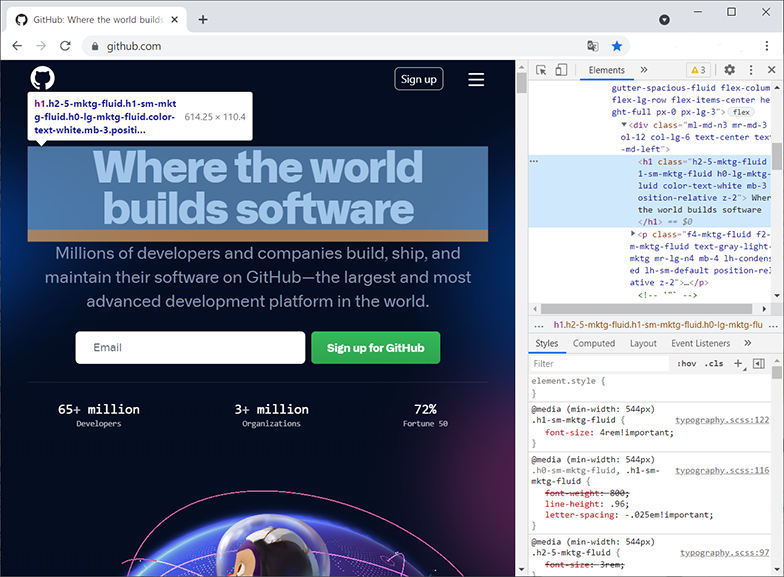
\includegraphics[width=\textwidth]{images/css-designing-html/chrome-devtools-layout.png}
        \caption{Chrome}
        \label{fig:devtools-chrome}
    \end{subfigure}
    \begin{subfigure}{.47\textwidth}\centering
        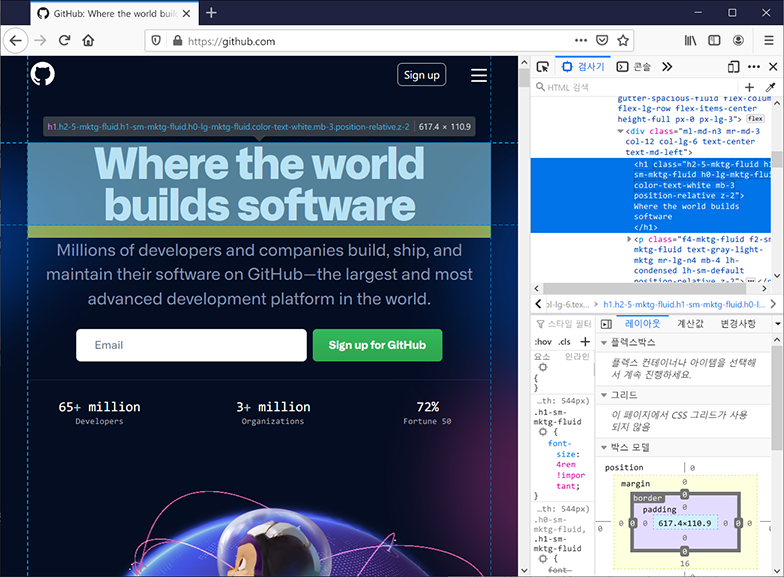
\includegraphics[width=\textwidth]{images/css-designing-html/firefox-devtools-layout.png}
        \caption{Firefox}
        \label{fig:devtools-firefox}
    \end{subfigure}
    \caption{Checking layout of HTML element using DevTools}
    \label{fig:devtools-layout}
\end{figure}

다행히도, 웹 브라우저의 개발자 도구는 특정한 HTML 요소가 웹 페이지 내에서 영역을 어떻게 차지하고 있으며, 어떻게 배치되었는지 확인할 수 있는 기능을 제공한다. Chrome과 Firefox에서 F12를 눌러 개발자 도구를 열고, Chrome은 Elements 탭을, Firefox는 검사기 탭을 눌러 열려있는 HTML 문서의 코드를 띄운다. 그리고 레이아웃을 확인하고자 하는 요소 위에 마우스를 hover하면 해당 요소의 레이아웃이 \figref{fig:devtools-layout}와 같이 나타난다. 반대로, 웹 페이지에서 HTML 코드를 확인하고 싶은 부분을 우클릭한 후 [검사]를 누르면 해당 요소의 코드를 찾아준다. 이렇게 HTML 문서를 작성할 때 개발자 도구를 이용하면 특정 요소가 어떠한 레이아웃을 갖는지, 어떻게 수정해야 할지 등의 정보를 보다 쉽게 얻을 수 있다.

\subsection*{Box Model}
HTML의 각 요소는 \textbf{사각형 형태}의 레이아웃을 가지며, 이러한 레이아웃을 box model이라고 한다. \figref{fig:box-model}을 참고하여 box model이 어떻게 구성되는지 알아보자.

\begin{itemize}
    \item Content: HTML 요소의 내용에 해당하는 부분이 배치되는 영역
    \begin{itemize}
        \item 예: \texttt{img} 태그의 이미지, 제목 태그의 내부 텍스트
    \end{itemize}
    \item Border: 요소의 테두리가 차지하는 영역
    \item Padding: Border과 content 사이의 영역
    \begin{itemize}
        \item 예: 배경은 content 영역과 padding 영역에 적용됨
    \end{itemize}
    \item Margin: 테두리 바깥쪽에서 요소가 차지하는 영역. 원칙상 다른 요소와는 겹치지 않음.
\end{itemize}

\figcmd{fig:box-model}{Box Model}{images/css-designing-html/box-model.png}{.15}

이 box model은 HTML 요소 배치의 기본이 되기 때문에 제대로 이해하는 것이 매우 중요하다. 앞으로 나오는 예제 코드를 직접 작성해보고, 브라우저의 개발자 도구를 이용하여 padding과 border, margin이 어떻게 나타나는지 각각 살펴보자.

먼저, content에 관여하는 속성으로는 \texttt{width}와 \texttt{height}가 있다. 두 속성은 각각 content 영역의 너비와 높이를 지정하는 속성이며, px, em 등의 단위나 \%를 이용하여 명시할 수 있다. \%로 지정하는 경우는 상위 요소의 너비나 높이를 기준으로 한다.

\begin{codeenv}{code:box-content-area}{Content Area}\begin{verbatim}
<style>
    #small-box {
        width: 400px;
        height: 200px;
        background-color: red;
    }

    #large-box {
        width: 800px;
        height: 400px;
        background-color: blue;
    }
</style>

<div id="small-box"></div>
<div id="large-box"></div>
\end{verbatim}
\end{codeenv}

Border에 관여하는 속성으로는 \texttt{border-width}, \texttt{border-style}, \texttt{border-color} 등이 있다. \texttt{border-height}는 테두리의 굵기, \texttt{border-style}은 테두리의 모양, \texttt{border-color}는 테두리의 색상을 나타내는 속성으로, 테두리의 모양은 \texttt{solid}, \texttt{dashed}, \texttt{dotted} 등의 값을 지정하여 테두리의 모양을 결정할 수 있다. 이 세가지 속성은 각각 따로 작성하여도 되고, \texttt{border} 속성에 굵기, 모양, 색상 순으로 나열하여 작성할 수도 있다. \coderef{code:box-border-area}에서 \texttt{\#box} 요소의 \texttt{border} 속성이 이러한 방법으로 작성되었다. 

또한, 방향에 관한 키워드\footnote{CSS에서 문서의 위, 아래, 왼쪽, 오른쪽 방향의 키워드는 각각 \texttt{top}, \texttt{bottom}, \texttt{left}, \texttt{right}이다.}를 사용하여 네 면 중 하나의 면에만 특정 스타일을 지정해줄 수 있다. 예를 들어, 왼쪽 면에만 스타일을 적용하고 싶은 경우 \texttt{border-left} 속성에 스타일을 작성한다.

\texttt{border-radius}는 테두리의 모서리를 둥글게 만들 수 있는 속성으로, 속성값이 하나인 경우 주어진 값을 반지름으로 하는 원형으로, 두 개인 경우 두 값을 짧은 반지름과 긴 반지름으로 하는 타원형으로 만든다. \texttt{border}와 마찬가지로 네 모서리에 모두 적용되며, 한쪽 모서리에만 적용하고 싶은 경우 역시 방향과 관련된 키워드를 사용하여 기술한다. 예를 들어, 좌상단 모서리의 스타일은 \texttt{border-top-left-radius} 속성에 작성한다.

\begin{codeenv}{code:box-border-area}{Border Area}\begin{verbatim}
<style>
    #box {
        width: 300px;
        height: 300px;
        border: 3px solid black;
        border-radius: 20px;
    }
</style>

<div id="box"></div>
\end{verbatim}
\end{codeenv}

Padding 속성은 border 영역의 각 면이 content 영역의 각 면으로부터 어느 정도 떨어져 있는지, margin 속성은 요소 가장자리의 각 면이 border 영역의 각 면으로부터 어느 정도 떨어져 있는지 명시하여 작성해준다. 앞의 border 영역과 마찬가지로 방향 키워드를 사용하여 한쪽 면에만 특정 padding/margin 값을 적용할 수 있다. (예: \texttt{padding-left}, \texttt{margin-bottom})

다만 \texttt{padding}과 \texttt{margin} 속성은 방향마다 속성과 속성값을 모두 작성하는 번거로운 방식 대신, \tblref{tab:padding-margin-shortened}의 Shortened Form과 같이 \texttt{padding}, \texttt{margin} 속성의 값에 차례대로 각 방향의 값을 나열하여 작성하는 것이 가능하다.

\begin{tblenv}
    {tab:padding-margin-shortened}
    {Shortened \texttt{padding} and \texttt{margin}}
    {
        >{\raggedright}m{0.3\textwidth}
        >{\centering}m{0.1\textwidth}
        >{\centering}m{0.1\textwidth}
        >{\centering}m{0.1\textwidth}
        >{\centering}m{0.1\textwidth}
    }
    \thickhline
    Shortened Form & top & right & bottom & left \tabularnewline
    \hline
    \texttt{padding/margin: A;} & A & A & A & A \tabularnewline
    \texttt{padding/margin: A B;} & A & B & A & B \tabularnewline
    \texttt{padding/margin: A B C;} & A & B & C & B \tabularnewline
    \texttt{padding/margin: A B C D;} & A & B & C & D \tabularnewline
    \thickhline
\end{tblenv}

\coderef{code:box-model-padding-margin}를 참고하여 \texttt{padding}과 \texttt{margin}을 정하는 방법을 이해하고, 개발자 도구를 이용하여 box model의 각 부분이 웹 브라우저상에 어떻게 표시되는지 확인해보자. 

\begin{codeenv}{code:box-model-padding-margin}{Examining Box Model}\begin{verbatim}
<style>
    .box {
        width: 100px;
        height: 200px;
        border: 2px dashed green;
        padding: 10px 20px;
        margin: 20px;
        background-color: orange;
        display: inline-block;         /* We will learn this later */
    }
</style>

<div class="box"></div>
<div class="box"></div>
<div class="box"></div>
<div class="box"></div>
<div class="box"></div>
\end{verbatim}
\end{codeenv}

\coderef{code:box-model-padding-margin}에서 \texttt{display: inline-block;}을 지우고 웹 페이지를 열어보면 각 \texttt{.box} 요소가 세로로 나열된다. 이때 \figref{fig:margin-collapsing}와 같이 두 요소의 margin이 겹친 것을 확인할 수 있으며, 이렇게 HTML 요소 간에 margin이 겹치는 현상을 마진 상쇄 또는 마진 겹침(margin collapsing)이라고 한다. Margin 겹침 현상은 인접한 형제 요소 간의 상하 margin이 겹칠 때, 빈 요소의 상하 margin이 겹칠 때, 부모 요소의 top(bottom) margin과 첫 번째(마지막) 자식 요소의 top(bottom) margin이 겹칠 때 발생한다. \coderef{code:box-model-padding-margin}의 경우는 형제 요소 간의 상하 margin이 겹친 경우로, 이러한 현상이 발생하는 디자인을 할 때 유의하여야 한다.

\begin{figure}[htb]\vspace{10pt}\centering
    \begin{subfigure}{.42\textwidth}\centering
        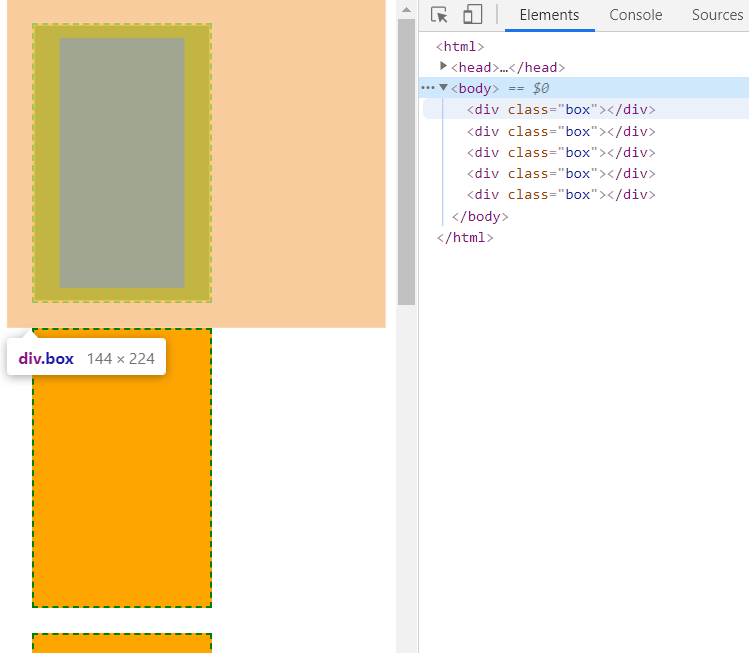
\includegraphics[width=\textwidth]{images/css-designing-html/margin-collapsing-upper-box.png}
        \caption{Upper Box}
        \label{fig:margin-collapsing-upper}
    \end{subfigure}
    \begin{subfigure}{.42\textwidth}\centering
        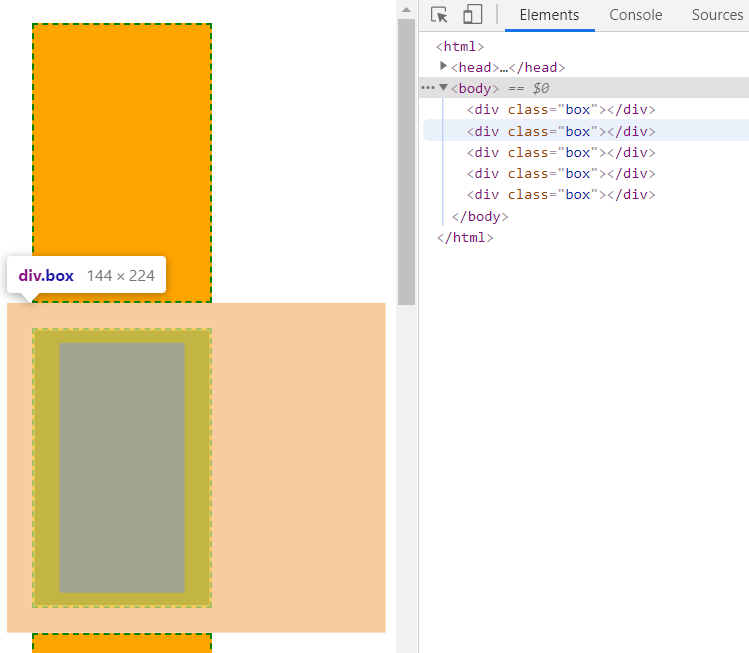
\includegraphics[width=\textwidth]{images/css-designing-html/margin-collapsing-lower-box.png}
        \caption{Lower Box}
        \label{fig:margin-collapsing-lower}
    \end{subfigure}
    \caption{Margin Collapsing}
    \label{fig:margin-collapsing}
\end{figure}

\subsection*{Inline-level and Block-level Elements}

지금까지 모든 HTML 요소는 box model에 따라 영역이 결정되고, 영역에 따라 다른 요소들과 맞물려 배치됨을 학습하였다. 앞의 \coderef{code:box-model-padding-margin}에서는 HTML 요소가 이전 형제 요소의 오른쪽에 충분히 빈 공간이 있다면 오른쪽에, 그렇지 않으면 아래쪽에 배치되었다. 그런데 지금까지 HTML을 다루면서, 이전 형제 요소에 따로 margin이나 padding을 지정해주지 않아도 이전 형제 요소와 같은 줄에 배치되지 않는 현상을 보았다.

\begin{codeenv}{code:inline-and-block-example}{Example of Inline-level, Block-level Elements}\begin{verbatim}
<h1>HTML Element Layout</h1>
<h2>This paragraph is about <span style="color: red">HTML element layout</span>.</h2>
\end{verbatim}
\end{codeenv}

\coderef{code:inline-and-block-example}에서 \texttt{h1} 태그와 \texttt{h2} 태그에 padding이나 margin이 전혀 부여되지 않았음에도 불구하고 서로 다른 줄에 배치되었다. 반대로, \texttt{h2} 태그 내부의 텍스트와 \texttt{span} 태그 내부의 텍스트는 서로 같은 줄에 배치되어 있다. 앞의 \sectref{sect:commonly-used-html-tags}에서 non-semantic 태그는 다른 요소와 같은 줄에 있으려고 하는지에 따라 \texttt{div} 태그와 \texttt{span} 태그로 나뉜다고 했던 것을 기억하는가? 이처럼 같은 줄에 다른 요소가 배치되는 것을 허용하는지에 따라 inline-level 요소와 block-level 요소로 구분할 수 있고, 이 성질은 \texttt{display} 속성을 이용하여 명시할 수 있다.

먼저 inline-level 요소는 다른 요소와 같은 줄을 공유하고, content의 너비만큼만 가로 폭을 차지한다. Inline-level 요소에는 \texttt{width}, \texttt{height}, \texttt{margin-top}, \texttt{margin-bottom}, \texttt{padding} 등의 속성을 적용할 수 없으며, 그 내부에 inline-level 요소를 포함할 수 없다. \texttt{display} 속성값이 \texttt{inline}인 요소는 inline-level 요소의 성질을 가지며, \texttt{span}, \texttt{a}, \texttt{strong}, \texttt{img}, \texttt{br}, \texttt{input}, \texttt{select}, \texttt{textarea}, \texttt{button} 등의 태그는 기본적으로 inline-level 요소이다. 

반대로 block-level 요소는 다른 요소와 같은 줄을 공유하지 않으며, 웹 페이지 화면의 가로 폭을 모두 차지하여 여러 block-level 요소들을 배치하면 수직 방향으로 배치된다. Block-level 요소에는 \texttt{width}, \texttt{height}, \texttt{margin}, \texttt{padding} 등의 속성을 적용할 수 있으며, 그 내부에 inline-level 요소를 포함할 수 있다. \texttt{display} 속성값을 \texttt{block}인 요소는 block-level 요소의 성질을 갖게 되며, \texttt{div}, \texttt{h1}\textasciitilde\texttt{h6}, \texttt{p}, \texttt{ol}, \texttt{ul}, \texttt{li}, \texttt{hr}, \texttt{table}, \texttt{form} 등의 태그는 기본적으로 block-level 요소이다.

그런데, 레이아웃을 구성하다 보면 요소들을 같은 줄에 배치하고 싶은데 \texttt{width}, \texttt{height}, \texttt{margin}, \texttt{padding} 등의 속성을 사용해야 하는 경우가 있다. 이러한 문제는 해당 요소의 \texttt{display} 값을 \texttt{inline-block}으로 지정하여 해결할 수 있다. \texttt{inline-block}은 inline-level 요소의 성질과 block-level 요소의 성질을 모두 갖는다. 또한, \texttt{display} 값을 \texttt{none}으로 지정하면 해당 요소가 보이지 않아, 사용자로부터 숨길 수 있다.\footnote{유사한 속성으로는 \texttt{visibility: hidden}이 있으나, \texttt{display: none}과는 달리 요소가 공간을 차지하되 보이지만 않게끔 한다.}
 
\coderef{code:box-model-padding-margin}에서 \texttt{display} 속성의 값을 바꿔보며 이해해보자. 

\subsection*{Position}

지금까지는 이전의 형제 요소가 배치되고 난 다음 공간에 다음 요소가 차례대로 배치되는 레이아웃 배치 방식에 대해 알아보았다. 이러한 방식이 일반적인 배치 방식이지만, 간혹 웹페이지에서 다른 요소들과의 위치와는 관계없이 고정된 위치에 배치되는 요소들이 있고, 다른 요소와 겹치게끔 배치되는 요소들이 있다. 대표적으로는 뉴스 기사에서 스크롤을 내려도 계속 화면상에 표시되는 광고들이 이러한 배치를 갖는다. 이렇게 특정 위치에 HTML 요소를 배치하고자 할때 \texttt{position} 속성을 이용한다.

\texttt{position} 속성에는 \texttt{static}, \texttt{relative}, \texttt{absolute}, \texttt{fixed}의 네 가지 값이 존재한다. 기본값은 \texttt{static}으로, \texttt{static} 배치 방식은 HTML 요소가 지금까지 학습해왔던 배치 방식, 즉 빈 공간에 왼쪽에서 오른쪽으로, 위에서 아래로 차례대로 배치된다. 나머지 세 값은 네 개의 방향 속성을 함께 사용하여 요소의 위치를 정할 수 있다. 방향 속성, 즉 \texttt{top}, \texttt{left}, \texttt{right}, \texttt{bottom} 속성은 기준점이 요소로부터 어떤 방향으로 얼마나 떨어져 있는지 나타내며, 속성값이 명시되지 않은 경우 기본값은 \texttt{0}이다.

먼저 \texttt{relative}는 \texttt{static}으로 지정되었을 때를 기준으로 방향 속성의 값에 따라 이동되어 배치되며, 네 방향 속성이 모두 지정되지 않은 경우 \texttt{static}과 동일하게 배치된다. \texttt{relative}로 인해 \texttt{static}이었을 때와 비교하여 요소의 위치가 벗어났다고 해서 다른 요소들의 위치가 바뀌는 것은 아니다.

\texttt{absolute}는 원래 요소가 배치되었어야 할 공간과 관계없이 \texttt{position} 값이 \texttt{static}이 아닌 부모나 조상 요소를 기준으로 배치되며, 이러한 부모나 조상 요소를 찾지 못하면 \texttt{body} 태그를 기준으로 배치된다. \texttt{absolute} 속성값을 갖는 요소가 원래 배치되었어야 하는 공간에는 다른 요소가 들어올 수 있으며, 요소의 \texttt{display} 속성이 \texttt{block}이더라도 너비가 content에 맞게 바뀌기 때문에 적절한 너비를 지정해주어야 한다.

\texttt{fixed}는 \texttt{absolute}와 유사한 성질을 갖지만, 위치를 지정하는 기준이 viewport, 즉 화면에 보여지는 웹페이지의 영역이다. 따라서 화면을 스크롤하여 올리거나 내렸을 때도 화면에서 고정된 위치에 요소를 배치할 때 사용된다.

 \coderef{code:position-property}에서 \texttt{\#pos-element}에 \texttt{position}에 관련된 속성과 그 값을 지정하고 바꿔가며 \texttt{position}에 대해 정확히 이해해보자.

\begin{codeenv}{code:position-property}{Example of \texttt{position} Property}\begin{verbatim}
<style>
    .box {
        width: 100px;
        height: 3000px;
        border: 1px solid;
        display: inline-block;
        background-color: skyblue;
        border-color: blue;
    }

    .red-box {
        height: 100px;
        background-color: pink;
        border-color: red;
    }

    #pos-element {
        /* Your CSS code here */
    }
</style>

<div class="box">1</div>
<div class="box red-box" id="pos-element">2</div>
<div class="box">3</div>
<div class="box">4</div>
\end{verbatim}
\end{codeenv}

여담으로, \texttt{position} 속성을 다루다 보면 요소 간에 겹침이 발생하여 특정 요소를 다른 요소 위에 오도록 할 필요가 있다. 이때 \texttt{z-index} 속성을 이용하면 요소 간의 쌓임 순서를 조절할 수 있다. \texttt{z-index}의 값은 정수(integer)이며, \texttt{0}이 기본값이고, 값이 높은 요소가 위에 쌓이고, 낮은 요소는 아래에 쌓인다. 
